\subsection{Angular moments analysis}
\label{sec:kpimm:angular-analysis}

The angular observables defined in Sec.~\ref{sec:kpimm:angular-distribution} are determined using a moments analysis of the angular distribution, as outlined in Ref.~\cite{biplab}. This approach has the advantage of producing stable measurements with well-defined uncertainties even for small data samples.

The 41 background-subtracted and acceptance-corrected moments are estimated as
\begin{equation}
 \label{eqn:moments}
\Gamma_i =  \sum_{k=1}^{n_{\rm sig}} w_{k}f_i(\Omega_k)  - x\sum_{k=1}^{n_{\rm bkg}} w_{k}f_i(\Omega_k)\\
\end{equation}

\noindent and the corresponding covariance matrix is estimated as

\begin{equation}
 \label{eqn:covariance}
 C_{ij} = \sum_{k=1}^{n_{\rm sig}} w^{2}_{k}f_i(\Omega_k)f_j(\Omega_k)   + x^2\sum_{k=1}^{n_{\rm bkg}} w^{2}_{k}f_i(\Omega_k)f_j(\Omega_k).
\end{equation}

\noindent Here $n_{\rm sig}$ and $n_{\rm bkg}$ correspond to the candidates in the signal and background regions, respectively. The signal region is defined within $\pm 50\mevcc$ of the mean \Bz mass, and the background region in the range $5350<\mkpimm<5700$~\mevcc.  The scale factor $x$ is the ratio of the estimated number of background candidates in the signal region over the number of candidates in the background region and is used to normalise the background subtraction.
It has been checked in data that the angular distribution of the background is independent of \mkpimm within the precision of this measurement, and that the uncertainty on $x$ has negligible impact on the results.
The weights, $w_{k}$, are the reciprocals of the candidates' efficiencies and account for the acceptance, described in Sec.~\ref{sec:kpimm:acceptance}.

The covariance matrix describing the statistical uncertainties on the 40 normalised moments is computed as
\begin{align}
\label{eqn:red_cov_def}
\overline{C}_{ij} = \left[C_{ij} + \frac{\Gamma_i \Gamma_j}{\Gamma_1^2} C_{11} - \frac{\Gamma_i C_{1j} + \Gamma_j C_{1i}}{\Gamma_1}\right] \frac{1}{\Gamma_1^2},  \;\; i,j \in \{2,...,41\}.
\end{align}

\subsubsection{Toy studies}
\label{sec:kpimm:angular-analysis:toys}

In order to validate the moments analysis, toy studies are performed using simulated datasets. Signal decays are generated according to a realistic model taking into account contributions from $K^\ast(1410)^0$~\cite{Zwicky-K_1_1410}, $K^\ast_0(1430)^0$~\cite{Wang-K_0_1430} and $K^\ast_2(1430)^0$~\cite{Wang-K_2_1430} states. The generated values for each of the moments are calculated using a numeric integration. The specified \mkpi and \qsq range is iterated over and the amplitudes at each point are calculated. The moments are then derived from these amplitudes using the relations given in Appendix~\ref{sec:appendix:angular-distribution}.

The toy datasets are generated in the range $1330<\mkpi<1530~\mevcc$ and $1.1<\qsq<6.0\gevgevcccc$. Each dataset contains a realistic amount of signal and background candidates, the numbers of which are both Poisson fluctuated. Background candidates are generated flat in \qsq, \ctl, \ctk, $\phi$, and \mkpi, and according to an exponential distribution in \mkpimm. Acceptance effects are also included using the efficiency function described in Sec.~\ref{sec:kpimm:acceptance}.
 
The 40 normalised moments $\overline{\Gamma}_{2}-\overline{\Gamma}_{41}$ are measured for each of the toy datasets. Pull studies are performed to check that the method is unbiased and correctly estimates the uncertainty. The results of the pull studies are shown in Table~\ref{table:spd:toy_pulls} and in Appendix~\ref{sec:appendix:kpimm:toys}. No significant bias is observed for any of the measured moments.

\begin{table}[!tb]
\caption{Results of the pull studies for toys datasets.}
\centering
\begin{tabular}{l|c|c}
$\overline{\Gamma}_{\it{i}}$ & mean & width \\ 
\hline
$\overline{\Gamma}_{2}$ & $-0.01$ $\pm$ 0.02 & $0.99$ $\pm$ 0.01 \\ 
$\overline{\Gamma}_{3}$ & $\hphantom{-}0.01$ $\pm$ 0.02 & $0.96$ $\pm$ 0.02 \\ 
$\overline{\Gamma}_{4}$ & $-0.03$ $\pm$ 0.02 & $0.95$ $\pm$ 0.02 \\ 
$\overline{\Gamma}_{5}$ & $-0.03$ $\pm$ 0.02 & $1.00$ $\pm$ 0.02 \\ 
$\overline{\Gamma}_{6}$ & $\hphantom{-}0.01$ $\pm$ 0.02 & $1.01$ $\pm$ 0.02 \\ 
$\overline{\Gamma}_{7}$ & $\hphantom{-}0.02$ $\pm$ 0.02 & $1.01$ $\pm$ 0.02 \\ 
$\overline{\Gamma}_{8}$ & $-0.01$ $\pm$ 0.02 & $0.97$ $\pm$ 0.02 \\ 
$\overline{\Gamma}_{9}$ & $-0.01$ $\pm$ 0.02 & $0.99$ $\pm$ 0.02 \\ 
$\overline{\Gamma}_{10}$ & $-0.03$ $\pm$ 0.02 & $0.97$ $\pm$ 0.02 \\ 
$\overline{\Gamma}_{11}$ & $\hphantom{-}0.01$ $\pm$ 0.02 & $0.94$ $\pm$ 0.02 \\ 
$\overline{\Gamma}_{12}$ & $-0.03$ $\pm$ 0.02 & $0.98$ $\pm$ 0.02 \\ 
$\overline{\Gamma}_{13}$ & $\hphantom{-}0.00$ $\pm$ 0.02 & $0.98$ $\pm$ 0.02 \\ 
$\overline{\Gamma}_{14}$ & $\hphantom{-}0.03$ $\pm$ 0.02 & $0.95$ $\pm$ 0.01 \\ 
$\overline{\Gamma}_{15}$ & $-0.01$ $\pm$ 0.02 & $0.97$ $\pm$ 0.01 \\ 
$\overline{\Gamma}_{16}$ & $\hphantom{-}0.00$ $\pm$ 0.02 & $0.97$ $\pm$ 0.02 \\ 
$\overline{\Gamma}_{17}$ & $\hphantom{-}0.03$ $\pm$ 0.02 & $1.01$ $\pm$ 0.02 \\ 
$\overline{\Gamma}_{18}$ & $-0.00$ $\pm$ 0.02 & $0.97$ $\pm$ 0.02 \\ 
$\overline{\Gamma}_{19}$ & $-0.01$ $\pm$ 0.02 & $1.00$ $\pm$ 0.02 \\ 
$\overline{\Gamma}_{20}$ & $-0.00$ $\pm$ 0.02 & $0.97$ $\pm$ 0.02 \\ 
$\overline{\Gamma}_{21}$ & $\hphantom{-}0.01$ $\pm$ 0.02 & $0.97$ $\pm$ 0.02 \\ 
\end{tabular}
\hspace{1em}
\begin{tabular}{c|c|c}
$\overline{\Gamma}_{\it{i}}$ & mean & width \\ 
\hline
$\overline{\Gamma}_{22}$ & $\hphantom{-}0.01$ $\pm$ 0.02 & $0.96$ $\pm$ 0.02 \\ 
$\overline{\Gamma}_{23}$ & $-0.01$ $\pm$ 0.02 & $0.96$ $\pm$ 0.02 \\ 
$\overline{\Gamma}_{24}$ & $-0.05$ $\pm$ 0.02 & $0.98$ $\pm$ 0.02 \\ 
$\overline{\Gamma}_{25}$ & $-0.01$ $\pm$ 0.02 & $0.99$ $\pm$ 0.02 \\ 
$\overline{\Gamma}_{26}$ & $-0.05$ $\pm$ 0.02 & $0.96$ $\pm$ 0.02 \\ 
$\overline{\Gamma}_{27}$ & $-0.01$ $\pm$ 0.02 & $0.96$ $\pm$ 0.02 \\ 
$\overline{\Gamma}_{28}$ & $-0.01$ $\pm$ 0.02 & $0.99$ $\pm$ 0.02 \\ 
$\overline{\Gamma}_{29}$ & $\hphantom{-}0.03$ $\pm$ 0.02 & $0.97$ $\pm$ 0.02 \\ 
$\overline{\Gamma}_{30}$ & $\hphantom{-}0.02$ $\pm$ 0.02 & $1.02$ $\pm$ 0.02 \\ 
$\overline{\Gamma}_{31}$ & $-0.00$ $\pm$ 0.02 & $0.97$ $\pm$ 0.01 \\ 
$\overline{\Gamma}_{32}$ & $\hphantom{-}0.00$ $\pm$ 0.02 & $1.01$ $\pm$ 0.02 \\ 
$\overline{\Gamma}_{33}$ & $-0.03$ $\pm$ 0.02 & $0.98$ $\pm$ 0.02 \\ 
$\overline{\Gamma}_{34}$ & $-0.00$ $\pm$ 0.02 & $0.98$ $\pm$ 0.02 \\ 
$\overline{\Gamma}_{35}$ & $-0.01$ $\pm$ 0.02 & $0.98$ $\pm$ 0.02 \\ 
$\overline{\Gamma}_{36}$ & $-0.00$ $\pm$ 0.02 & $0.96$ $\pm$ 0.01 \\ 
$\overline{\Gamma}_{37}$ & $-0.01$ $\pm$ 0.02 & $0.97$ $\pm$ 0.02 \\ 
$\overline{\Gamma}_{38}$ & $\hphantom{-}0.02$ $\pm$ 0.02 & $0.95$ $\pm$ 0.02 \\ 
$\overline{\Gamma}_{39}$ & $\hphantom{-}0.01$ $\pm$ 0.02 & $0.96$ $\pm$ 0.01 \\ 
$\overline{\Gamma}_{40}$ & $\hphantom{-}0.02$ $\pm$ 0.02 & $0.99$ $\pm$ 0.02 \\ 
$\overline{\Gamma}_{41}$ & $-0.01$ $\pm$ 0.02 & $0.96$ $\pm$ 0.02 \\ 
\end{tabular}
\label{table:spd:toy_pulls}
\end{table}

%\subsubsection{Consistency relations}

\subsubsection{F-wave moments}

The angular analysis assumes that the $\Kp\pim$ system is in a S-, P- or D-wave configuration only. Contributions from F-wave states (or higher) are assumed to be negligible. This assumption is cross-checked by measuring the 18 moments corresponding to the $\Kp\pim$ in a F-wave configuration. The measured values are shown in Fig.~\ref{fig:kpimm:angular-analysis:f-wave:fig} and Table~\ref{fig:kpimm:angular-analysis:f-wave:tab}. All the measured moments are consistent with zero.

\begin{figure}[!htb]
\caption{Results of the cross-check of the F-wave contribution. All the measured moments are consistent with zero.}
\centering
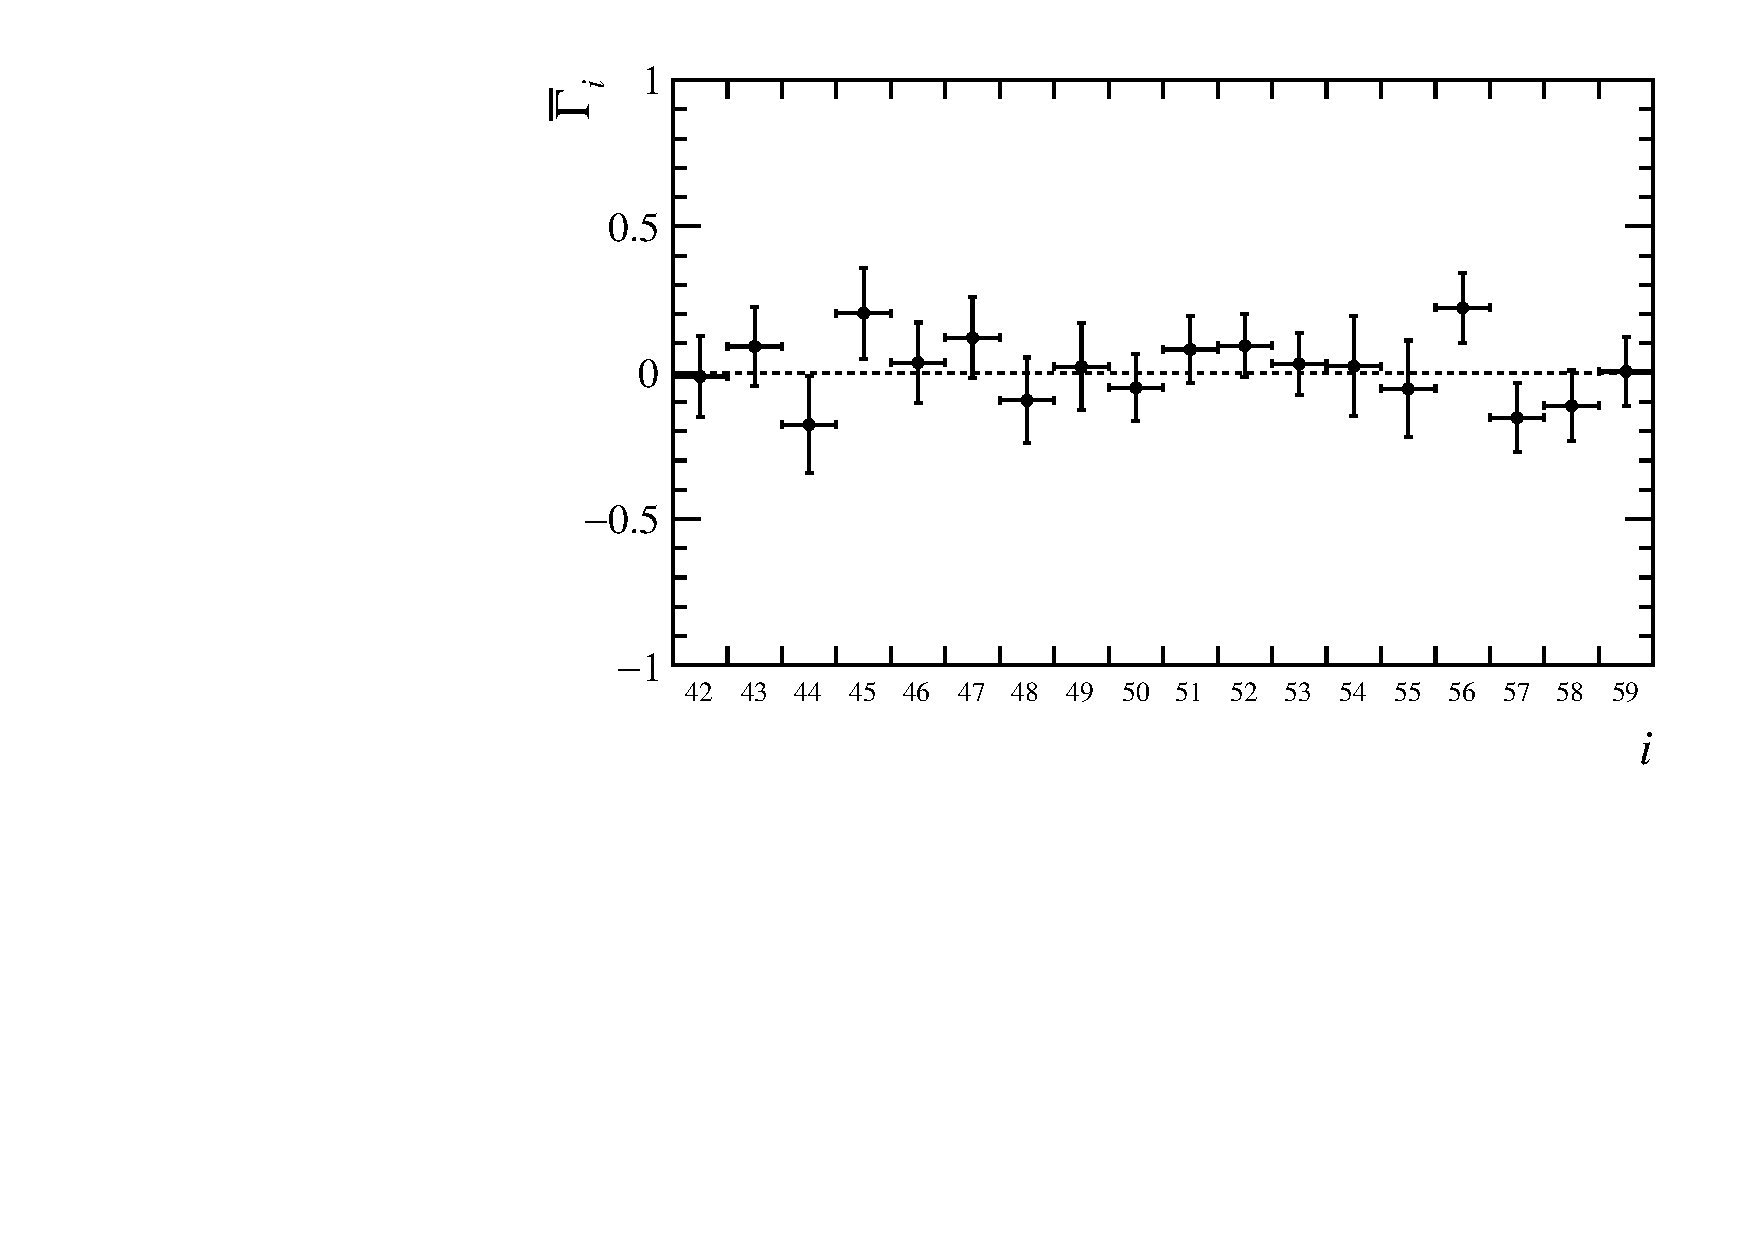
\includegraphics[width=0.7\textwidth]{figs/kpimm/angular-analysis/f-wave-moments.pdf}
\label{fig:kpimm:angular-analysis:f-wave:fig}
\end{figure}

\begin{table}[!htb]
\centering
\begin{tabular}{l|c|c}
& $f_{i}(\Omega)$ & Value \\
\hline
$\overline{\Gamma}_{42}$ & $P_{5}^{0}Y_{0}^{0}$ & $-0.01$ $\pm$ 0.14 \\ 
$\overline{\Gamma}_{43}$ & $P_{6}^{0}Y_{0}^{0}$ & \hphantom{$-$}0.09 $\pm$ 0.13 \\ 
$\overline{\Gamma}_{44}$ & $P_{5}^{0}Y_{2}^{0}$ & $-0.18$ $\pm$ 0.17 \\ 
$\overline{\Gamma}_{45}$ & $P_{6}^{0}Y_{2}^{0}$ & \hphantom{$-$}0.20 $\pm$ 0.16 \\ 
$\overline{\Gamma}_{46}$ & $P_{5}^{1}\sqrt{2}\rel(Y_{2}^{1})$ & \hphantom{$-$}0.03 $\pm$ 0.14 \\ 
$\overline{\Gamma}_{47}$ & $P_{6}^{1}\sqrt{2}\rel(Y_{2}^{1})$ & \hphantom{$-$}0.12 $\pm$ 0.14 \\ 
$\overline{\Gamma}_{48}$ & $P_{5}^{1}\sqrt{2}\img(Y_{2}^{1})$ & $-0.09$ $\pm$ 0.15 \\ 
$\overline{\Gamma}_{49}$ & $P_{6}^{1}\sqrt{2}\img(Y_{2}^{1})$ & \hphantom{$-$}0.02 $\pm$ 0.15 \\ 
$\overline{\Gamma}_{50}$ & $P_{5}^{0}\sqrt{2}\rel(Y_{2}^{2})$ & $-0.05$ $\pm$ 0.11 \\ 
$\overline{\Gamma}_{51}$ & $P_{6}^{0}\sqrt{2}\rel(Y_{2}^{2})$ & \hphantom{$-$}0.08 $\pm$ 0.11 \\ 
$\overline{\Gamma}_{52}$ & $P_{5}^{0}\sqrt{2}\img(Y_{2}^{2})$ & \hphantom{$-$}0.09 $\pm$ 0.11 \\ 
$\overline{\Gamma}_{53}$ & $P_{6}^{0}\sqrt{2}\img(Y_{2}^{2})$ & \hphantom{$-$}0.03 $\pm$ 0.11 \\ 
$\overline{\Gamma}_{54}$ & $P_{5}^{0}Y_{1}^{0}$ & \hphantom{$-$}0.02 $\pm$ 0.17 \\ 
$\overline{\Gamma}_{55}$ & $P_{6}^{0}Y_{1}^{0}$ & $-0.06$ $\pm$ 0.17 \\ 
$\overline{\Gamma}_{56}$ & $P_{5}^{1}\sqrt{2}\rel(Y_{1}^{1})$ & \hphantom{$-$}0.22 $\pm$ 0.12 \\ 
$\overline{\Gamma}_{57}$ & $P_{6}^{1}\sqrt{2}\rel(Y_{1}^{1})$ & $-0.15$ $\pm$ 0.12 \\ 
$\overline{\Gamma}_{58}$ & $P_{5}^{1}\sqrt{2}\img(Y_{1}^{1})$ & $-0.11$ $\pm$ 0.12 \\ 
$\overline{\Gamma}_{59}$ & $P_{6}^{1}\sqrt{2}\img(Y_{1}^{1})$ & \hphantom{$-$}0.00 $\pm$ 0.12 \\ 
\end{tabular}
\caption{Results of the cross-check of the F-wave contribution. All the measured moments are consistent with zero.}
\label{fig:kpimm:angular-analysis:f-wave:tab}
\end{table}

\subsubsection{Results}

The results for the normalised moments, $\overline{\Gamma}_{i}$, are given in Fig.~\ref{fig:results:moments}. The uncertainties shown are the sums in quadrature of the statistical and systematic uncertainties. The results are also presented in Table~\ref{tab:results:moments}. The various sources of the systematic uncertainties are described in Sec.~\ref{sec:kpimm:systematics}.

\begin{figure}[!tb]
\centering
  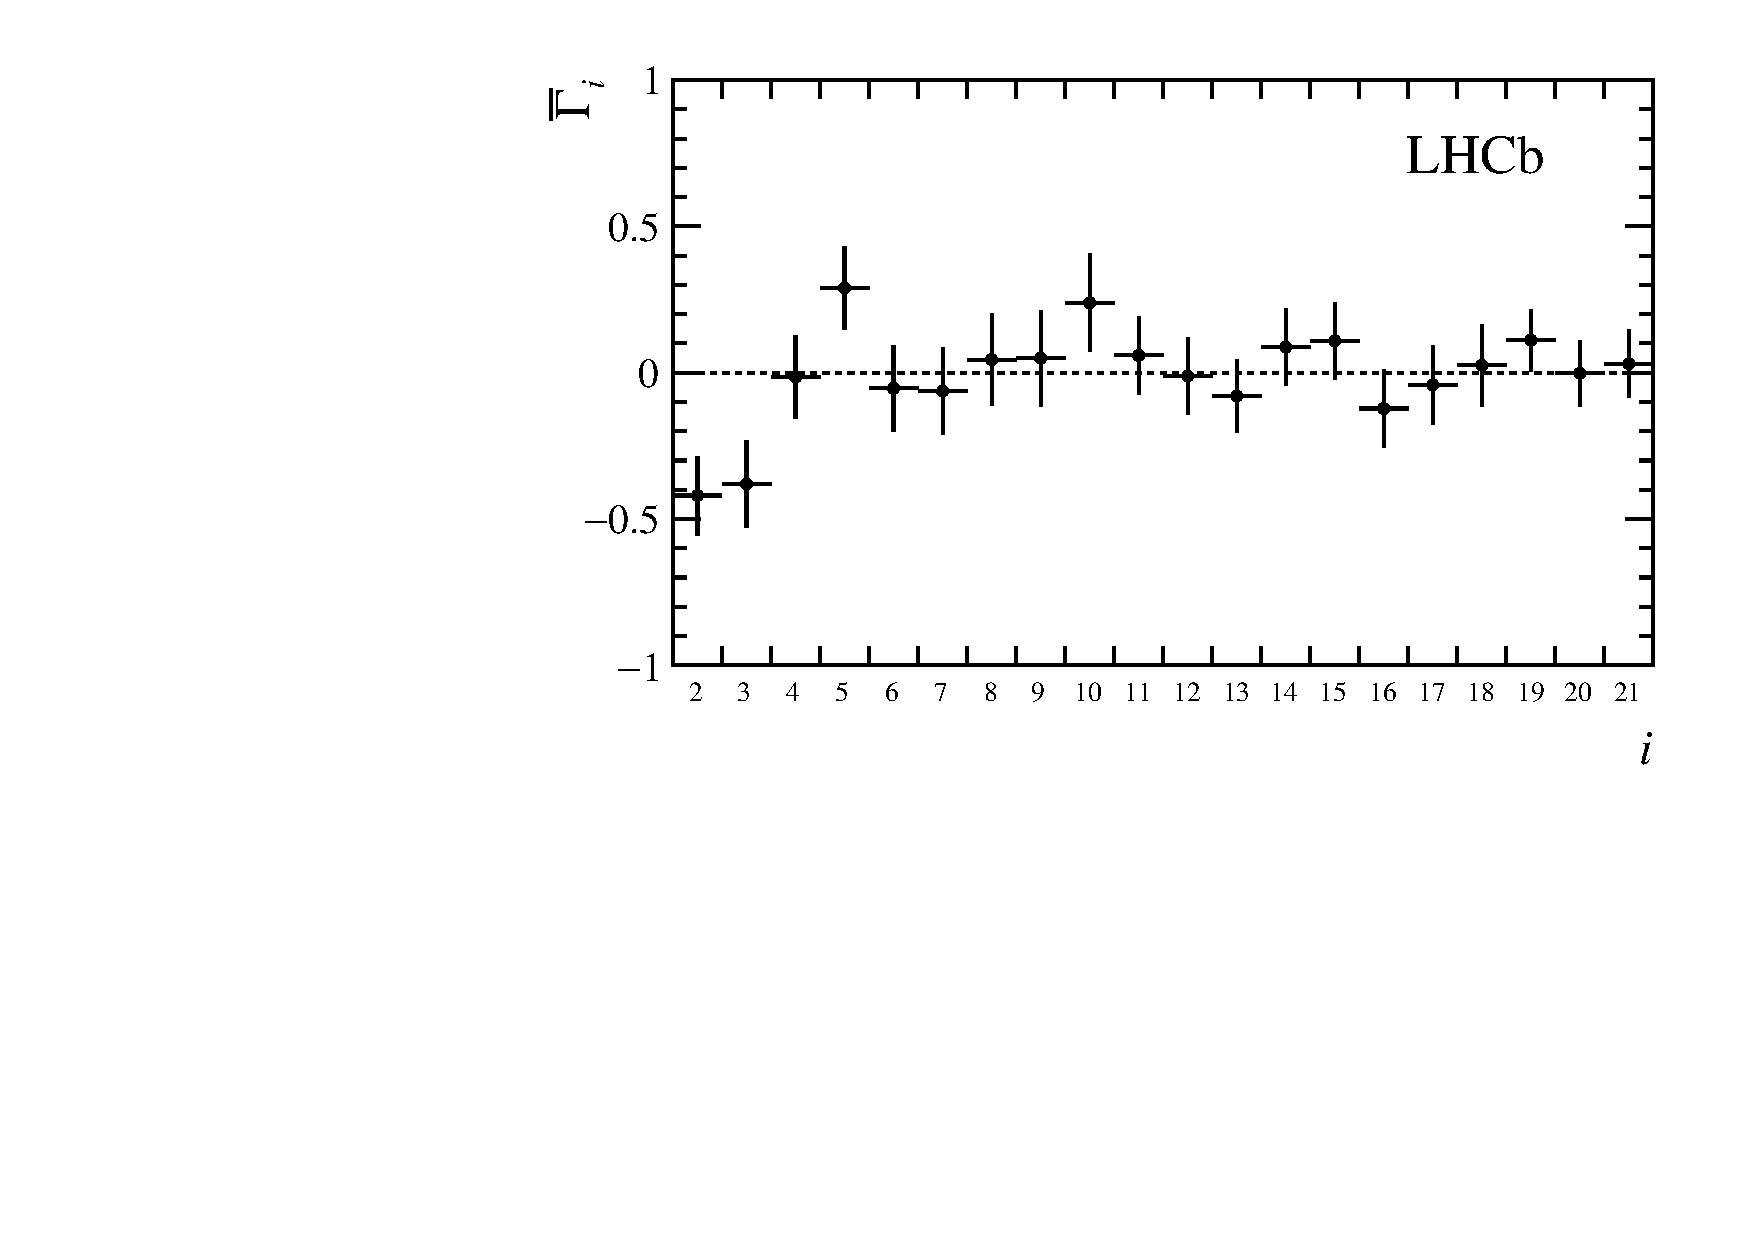
\includegraphics[width=0.7\textwidth]{figs/kpimm/angular-analysis/mom_results_2_21.pdf}
  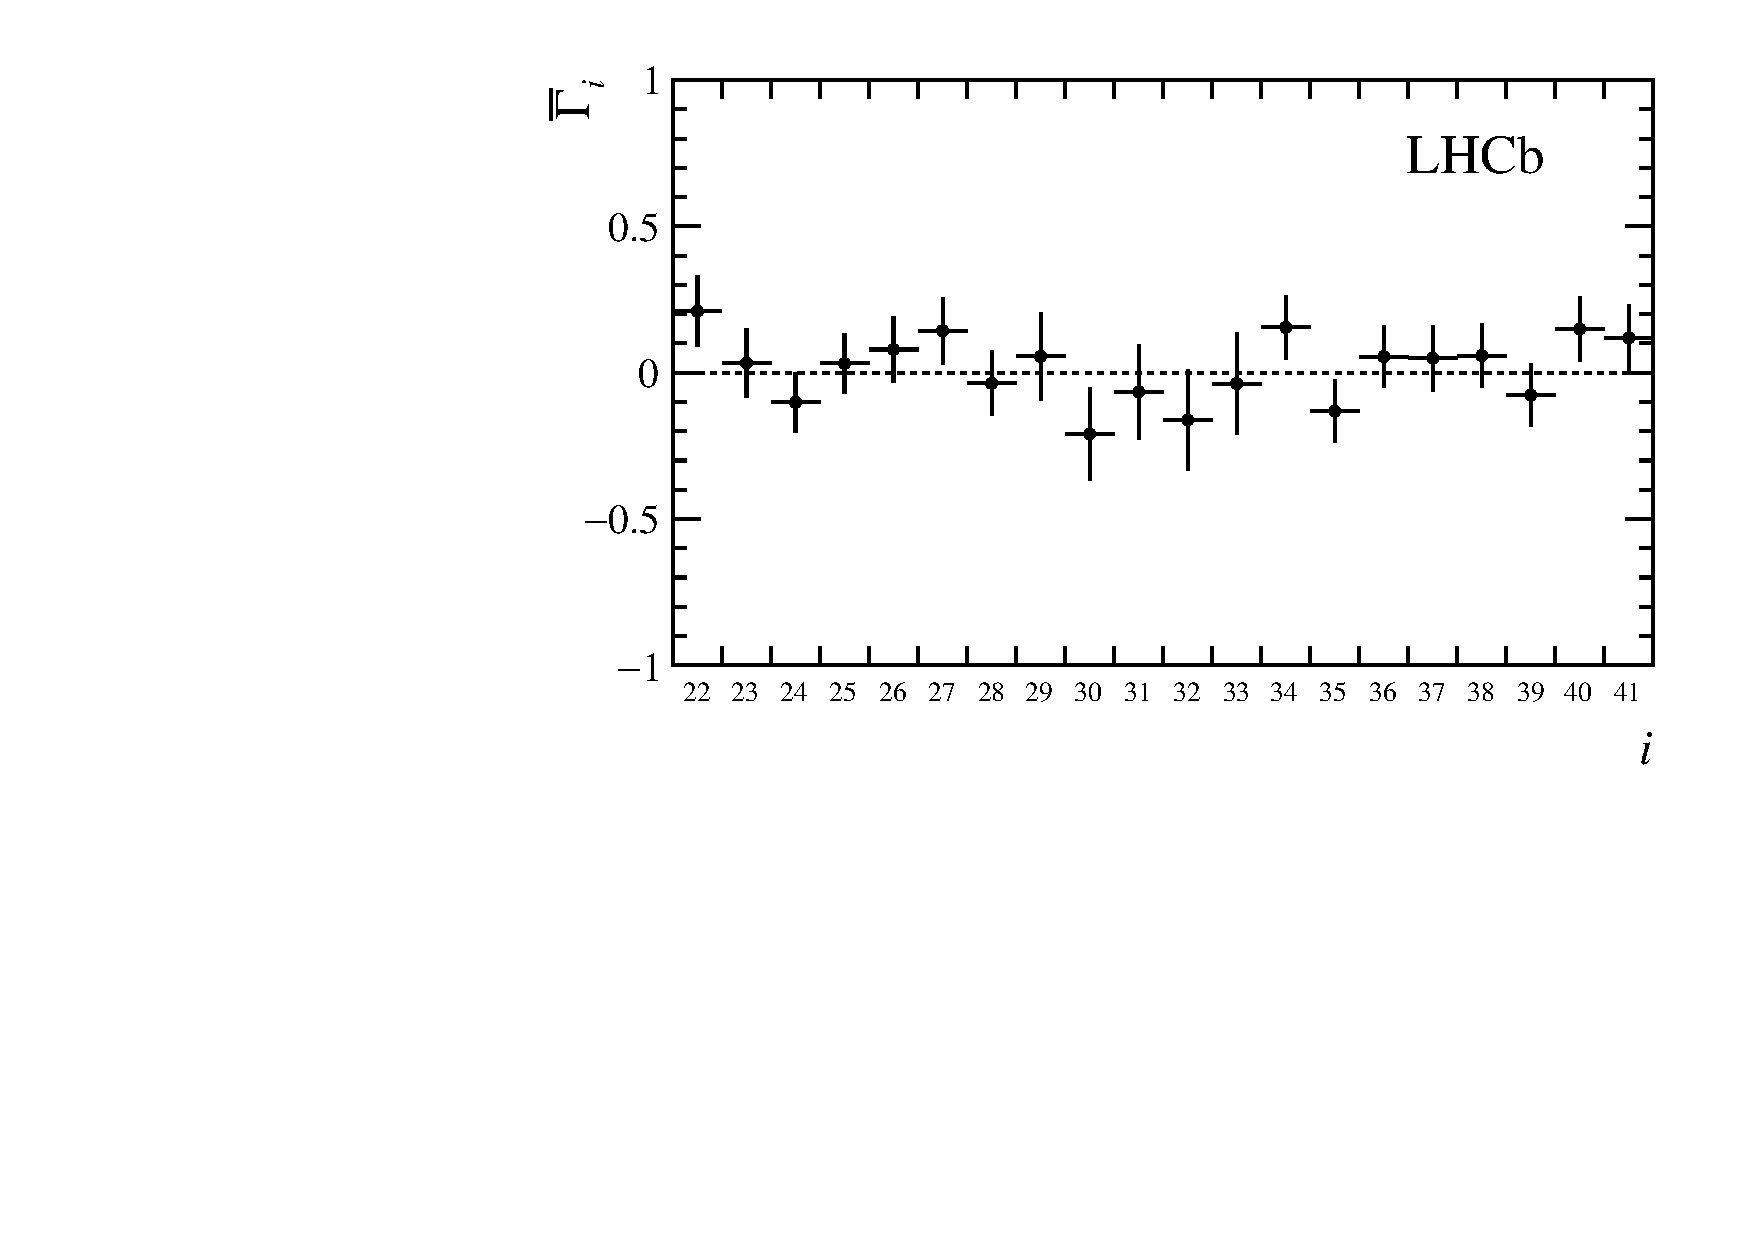
\includegraphics[width=0.7\textwidth]{figs/kpimm/angular-analysis/mom_results_22_41.pdf}
  \caption{Measurement of the normalised moments, $\overline{\Gamma}_{i}$, of the decay \BdToKpimm in the range $1.1<\qsq<6.0\gevgevcccc$ and $1330<\mkpi<1530\mevcc$. The uncertainties shown are the quadratic sum of the statistical and systematic uncertainties.}
  \label{fig:results:moments}
\end{figure}

\begin{table}[!tb]
\caption{Measurement of the normalised moments, $\overline{\Gamma}_{i}$, of the decay \BdToKpimm in the range $1.1<\qsq<6.0\gevgevcccc$ and $1330<\mkpi<1530\mevcc$. The first uncertainty is statistical and the second systematic.}
\label{tab:results:moments}
\centering
\begin{tabular}{l|c}
$\overline{\Gamma}_{i}$ & Value \\ 
\hline
$\overline{\Gamma}_{2}$ & $-0.42$ $\pm$ 0.13 $\pm$ 0.03 \\ 
$\overline{\Gamma}_{3}$ & $-0.38$ $\pm$ 0.15 $\pm$ 0.01 \\ 
$\overline{\Gamma}_{4}$ & $-0.02$ $\pm$ 0.14 $\pm$ 0.01 \\ 
$\overline{\Gamma}_{5}$ & \hphantom{$-$}0.29 $\pm$ 0.14 $\pm$ 0.02 \\ 
$\overline{\Gamma}_{6}$ & $-0.05$ $\pm$ 0.14 $\pm$ 0.04 \\ 
$\overline{\Gamma}_{7}$ & $-0.06$ $\pm$ 0.15 $\pm$ 0.03 \\ 
$\overline{\Gamma}_{8}$ & \hphantom{$-$}0.04 $\pm$ 0.16 $\pm$ 0.01 \\ 
$\overline{\Gamma}_{9}$ & \hphantom{$-$}0.05 $\pm$ 0.16 $\pm$ 0.02 \\ 
$\overline{\Gamma}_{10}$ & \hphantom{$-$}0.24 $\pm$ 0.17 $\pm$ 0.02 \\ 
$\overline{\Gamma}_{11}$ & \hphantom{$-$}0.06 $\pm$ 0.13 $\pm$ 0.01 \\ 
$\overline{\Gamma}_{12}$ & $-0.01$ $\pm$ 0.13 $\pm$ 0.02 \\ 
$\overline{\Gamma}_{13}$ & $-0.08$ $\pm$ 0.12 $\pm$ 0.01 \\ 
$\overline{\Gamma}_{14}$ & \hphantom{$-$}0.09 $\pm$ 0.13 $\pm$ 0.01 \\ 
$\overline{\Gamma}_{15}$ & \hphantom{$-$}0.11 $\pm$ 0.13 $\pm$ 0.00 \\ 
$\overline{\Gamma}_{16}$ & $-0.12$ $\pm$ 0.13 $\pm$ 0.01 \\ 
$\overline{\Gamma}_{17}$ & $-0.04$ $\pm$ 0.13 $\pm$ 0.01 \\ 
$\overline{\Gamma}_{18}$ & \hphantom{$-$}0.03 $\pm$ 0.14 $\pm$ 0.01 \\ 
$\overline{\Gamma}_{19}$ & \hphantom{$-$}0.11 $\pm$ 0.11 $\pm$ 0.01 \\ 
$\overline{\Gamma}_{20}$ & $-0.00$ $\pm$ 0.11 $\pm$ 0.01 \\ 
$\overline{\Gamma}_{21}$ & \hphantom{$-$}0.03 $\pm$ 0.12 $\pm$ 0.01 \\ 
\end{tabular}
\hspace{1em}
\begin{tabular}{l|c}
$\overline{\Gamma}_{i}$ & Value \\ 
\hline
$\overline{\Gamma}_{22}$ & \hphantom{$-$}0.21 $\pm$ 0.12 $\pm$ 0.01 \\ 
$\overline{\Gamma}_{23}$ & \hphantom{$-$}0.03 $\pm$ 0.12 $\pm$ 0.01 \\ 
$\overline{\Gamma}_{24}$ & $-0.10$ $\pm$ 0.10 $\pm$ 0.01 \\ 
$\overline{\Gamma}_{25}$ & \hphantom{$-$}0.03 $\pm$ 0.10 $\pm$ 0.01 \\ 
$\overline{\Gamma}_{26}$ & \hphantom{$-$}0.08 $\pm$ 0.11 $\pm$ 0.01 \\ 
$\overline{\Gamma}_{27}$ & \hphantom{$-$}0.14 $\pm$ 0.11 $\pm$ 0.01 \\ 
$\overline{\Gamma}_{28}$ & $-0.04$ $\pm$ 0.11 $\pm$ 0.01 \\ 
$\overline{\Gamma}_{29}$ & \hphantom{$-$}0.06 $\pm$ 0.15 $\pm$ 0.04 \\ 
$\overline{\Gamma}_{30}$ & $-0.21$ $\pm$ 0.15 $\pm$ 0.04 \\ 
$\overline{\Gamma}_{31}$ & $-0.07$ $\pm$ 0.16 $\pm$ 0.01 \\ 
$\overline{\Gamma}_{32}$ & $-0.16$ $\pm$ 0.17 $\pm$ 0.02 \\ 
$\overline{\Gamma}_{33}$ & $-0.04$ $\pm$ 0.17 $\pm$ 0.02 \\ 
$\overline{\Gamma}_{34}$ & \hphantom{$-$}0.15 $\pm$ 0.11 $\pm$ 0.01 \\ 
$\overline{\Gamma}_{35}$ & $-0.13$ $\pm$ 0.11 $\pm$ 0.01 \\ 
$\overline{\Gamma}_{36}$ & \hphantom{$-$}0.05 $\pm$ 0.11 $\pm$ 0.01 \\ 
$\overline{\Gamma}_{37}$ & \hphantom{$-$}0.05 $\pm$ 0.11 $\pm$ 0.01 \\ 
$\overline{\Gamma}_{38}$ & \hphantom{$-$}0.06 $\pm$ 0.11 $\pm$ 0.00 \\ 
$\overline{\Gamma}_{39}$ & $-0.08$ $\pm$ 0.11 $\pm$ 0.00 \\ 
$\overline{\Gamma}_{40}$ & \hphantom{$-$}0.15 $\pm$ 0.11 $\pm$ 0.01 \\ 
$\overline{\Gamma}_{41}$ & \hphantom{$-$}0.12 $\pm$ 0.11 $\pm$ 0.01 \\ 
\end{tabular}
\end{table}

The distributions of each of the decay angles within the signal region are shown in Fig.~\ref{fig:gof_spd}. The estimated signal distribution is derived 
from the moments model by evaluating the sum in Eq.~\ref{eqn:vector_moments}, which is found to provide a good representation of the data for each of the decay angles.

\begin{figure}[!tb]
  \centering
  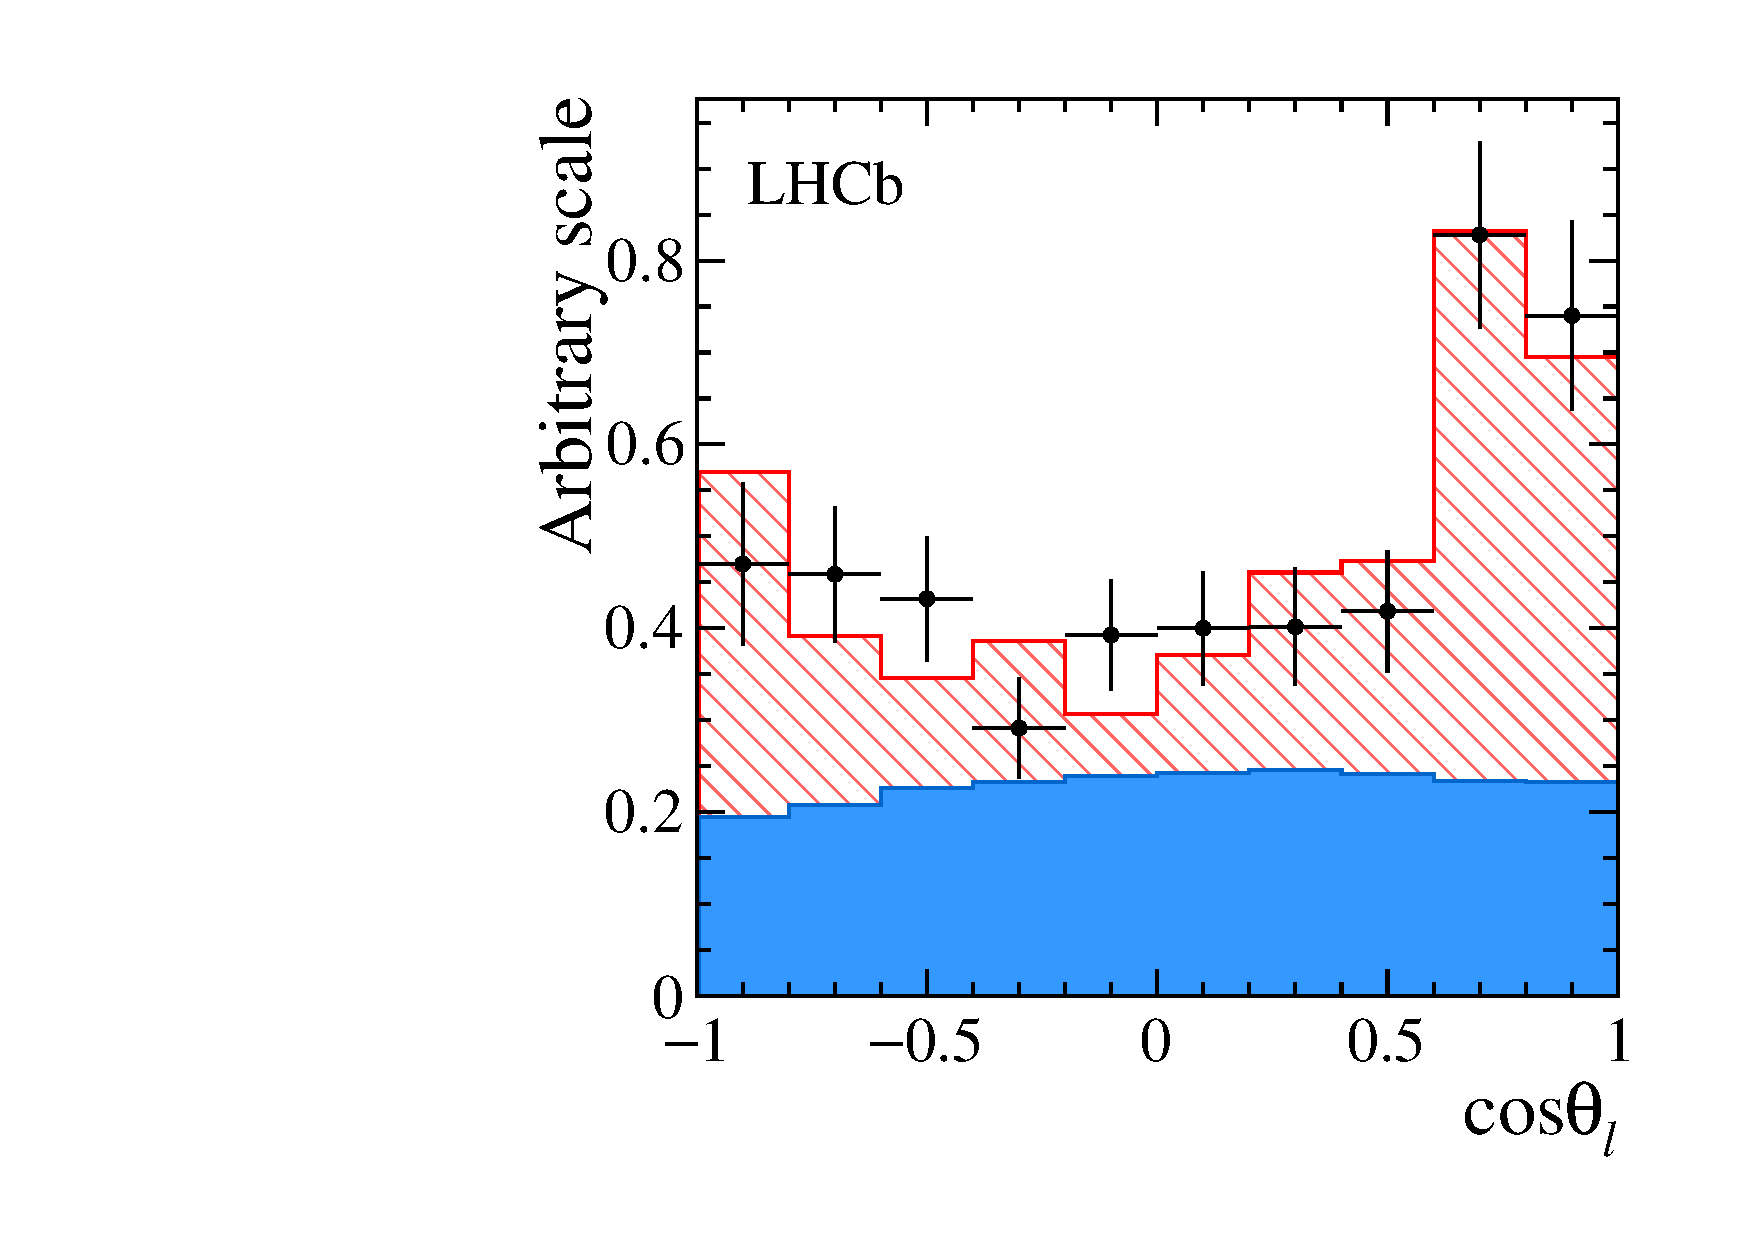
\includegraphics[width=0.45\textwidth]{figs/kpimm/angular-analysis/costhetal.pdf}
  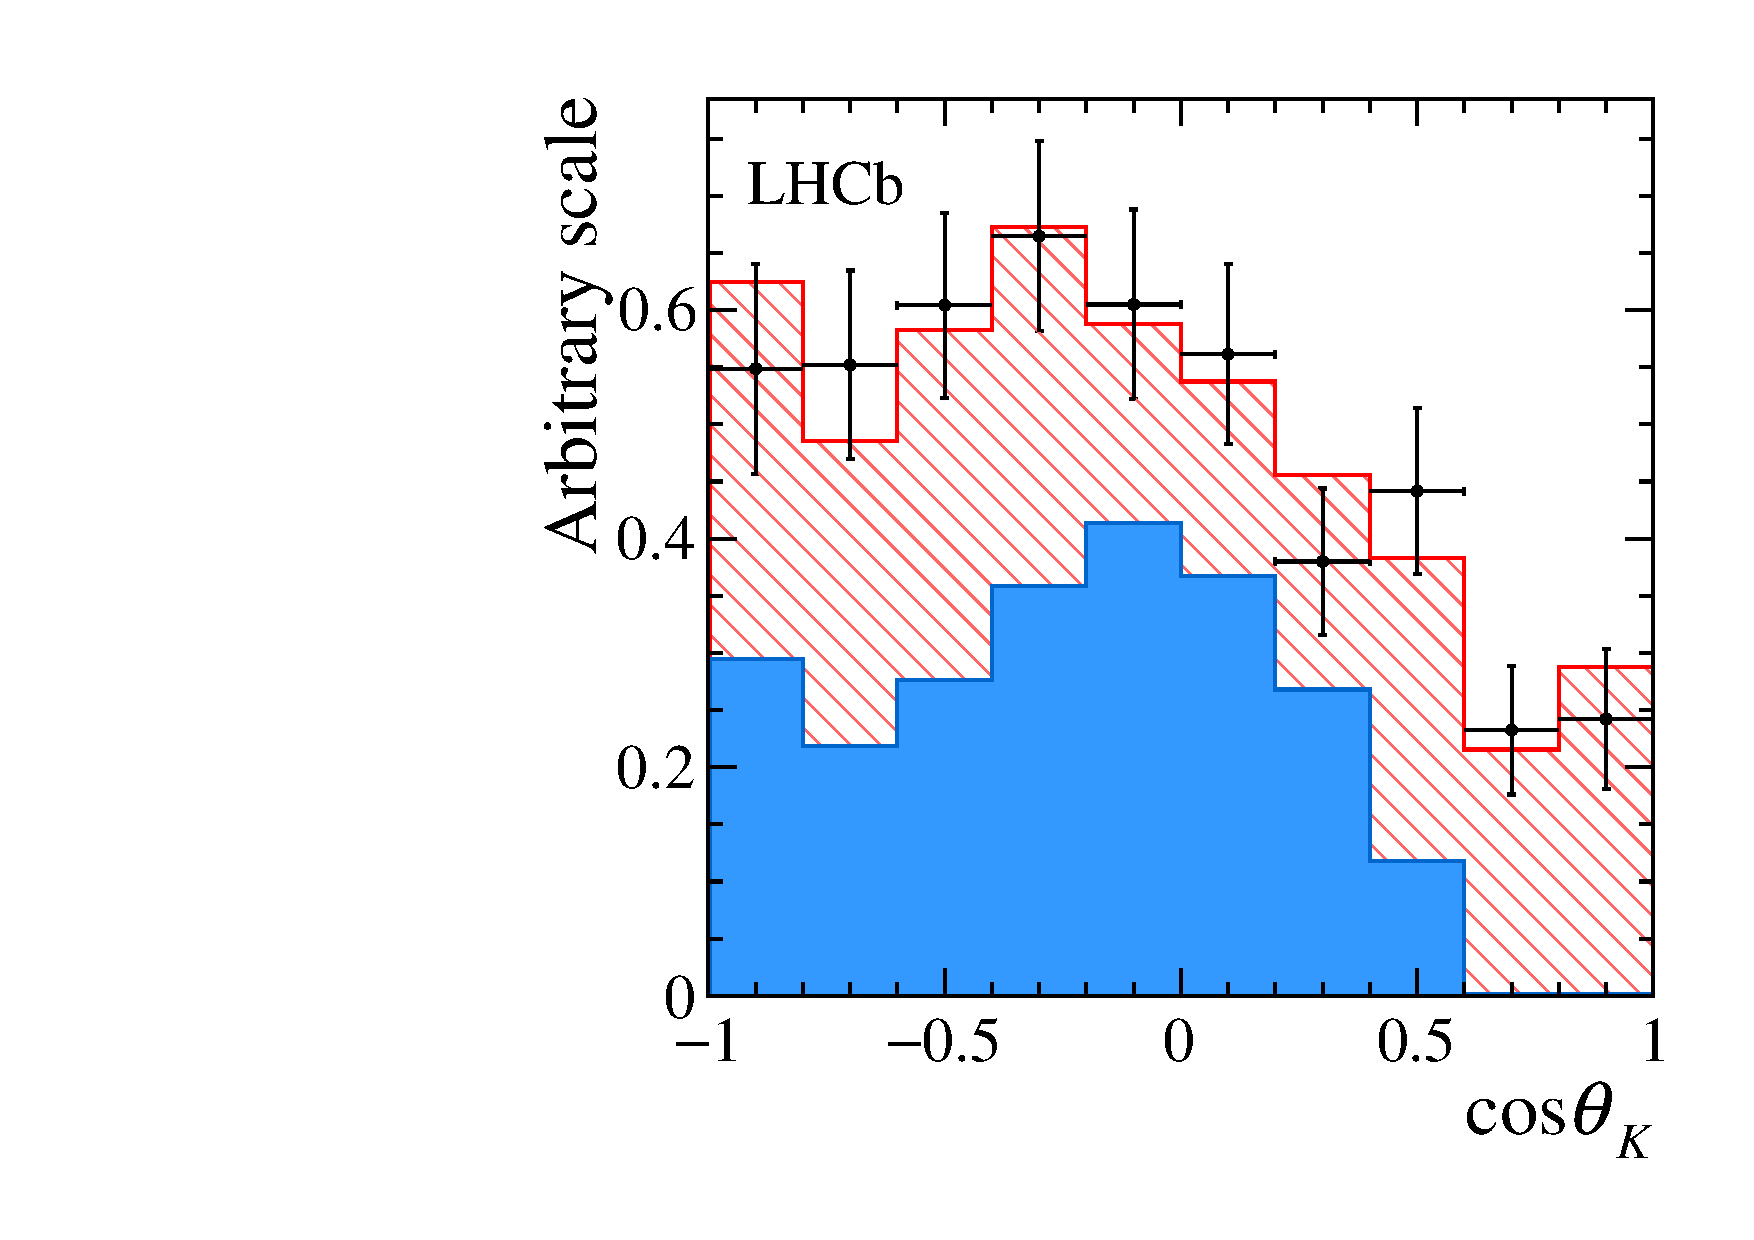
\includegraphics[width=0.45\textwidth]{figs/kpimm/angular-analysis/costhetak.pdf}\\
  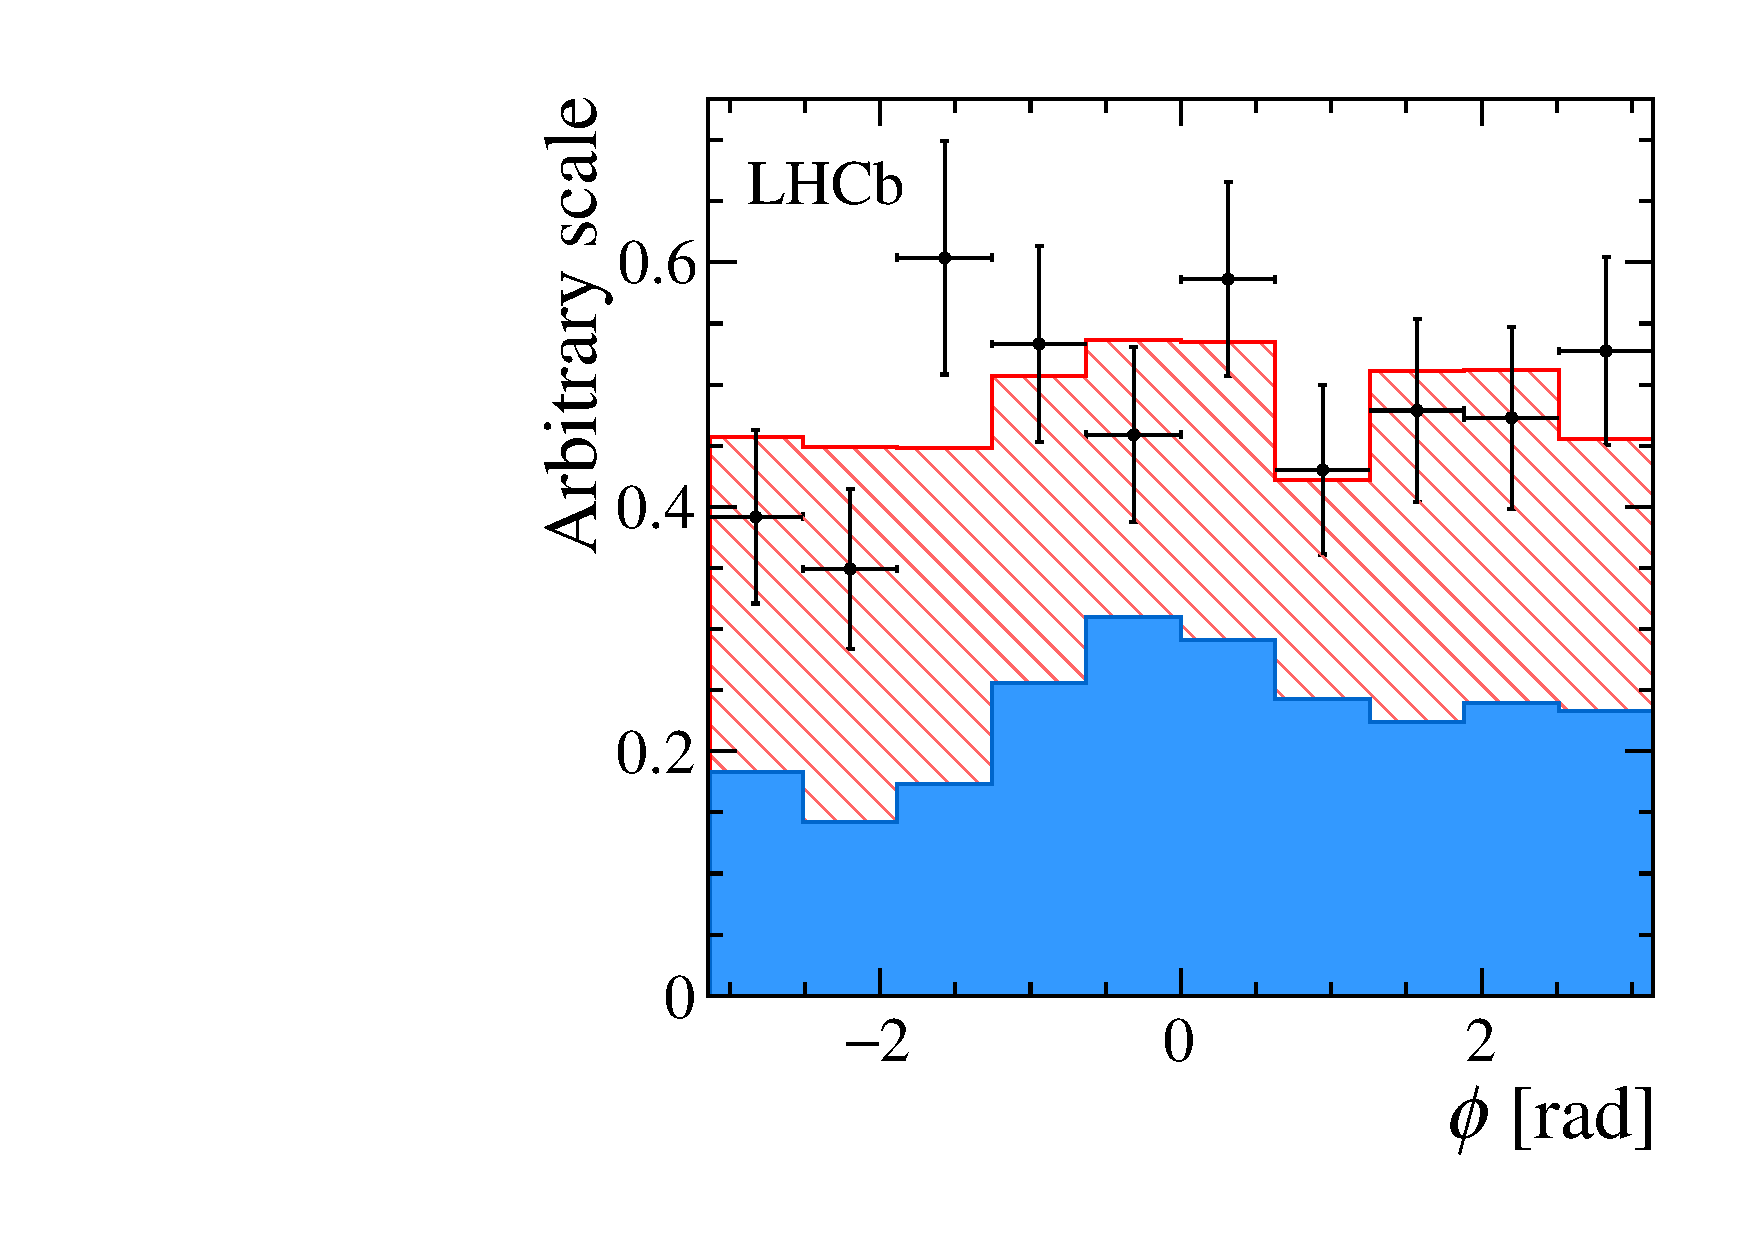
\includegraphics[width=0.45\textwidth]{figs/kpimm/angular-analysis/phi.pdf}
  \caption{The distributions of each of the decay angles within the signal region. The acceptance-corrected data is represented by the points with error bars. The estimated signal distribution is shown by the blue shaded histogram. The projected background from the upper mass sideband is shown by the red hatched histogram, which is stacked onto the signal histogram.}
  \label{fig:gof_spd}
\end{figure}

The D-wave fraction, $F_{\rm D}$, is estimated using the moments $\overline{\Gamma}_{5}$ and $\overline{\Gamma}_{10}$ as 

\begin{equation}
F_{\rm D} \equiv  \displaystyle - \frac{7}{18} \left(2 \overline{\Gamma}_{5} + 5 \sqrt{5} \overline{\Gamma}_{10} \right).
\end{equation}

\noindent
The D-wave fraction, $F_{\rm D}$, is estimated from the moments $\overline{\Gamma}_{5}$ and $\overline{\Gamma}_{10}$ as 

\begin{equation}
F_{\rm D} =  \displaystyle - \frac{7}{18} \left(2 \overline{\Gamma}_{5} + 5 \sqrt{5} \overline{\Gamma}_{10} \right).
\end{equation}

\noindent
Naively, one would expect a large D-wave contribution in this region, as was seen in the amplitude analysis of \BdToJPsiKpi~\cite{belle-z-paper}. However, in \BdToKpimm no significant D-wave contribution is seen and, with the limited statistics currently available, it is only possible to set an upper limit of $F_{\rm D}<0.29$ at 95\% confidence level. This might be an indication of a large breaking of QCD factorisation in this decay mode.  Additionally, the values of the moments $\overline{\Gamma}_{2}$ and $\overline{\Gamma}_{3}$ imply the presence of large interference effects between the S- and P- or D-wave contributions.